\chapter{Fall Response}\label{comparisonLinModelReal} 
\textbf{Name: Group 630}\\
\textbf{Date: 07/03 - 2016}

\subsubsection{Purpose}
Find the fall response of the frame from the vertical position, \si{\theta_F=0}\fxnote{might change depending on what is decided as the "real" 0 because of potmeter offset}, and from a \si{10^\circ}\fxnote{Might chance depending on data } tilted position. During this the wheel will be in a fixed position.

Data from this is used to compare the response of the real setup with the simulation given by the theoretical linearized model.

\subsubsection{Setup}
The wheel is being held in a fixed position with a strip tied to it and the frame. The probe chosen is a 1:1 and is connected to the potentiometer with probe to yellow cable and ground clamp to brown cable. The power supply has to be connected, and turned on, to the Cubli in order to get readouts from the potentiometer. A sponge is placed on the rubber pad in order to dampen the impact of the frame.
\begin{figure}[H]                                   
	\centering                                        
	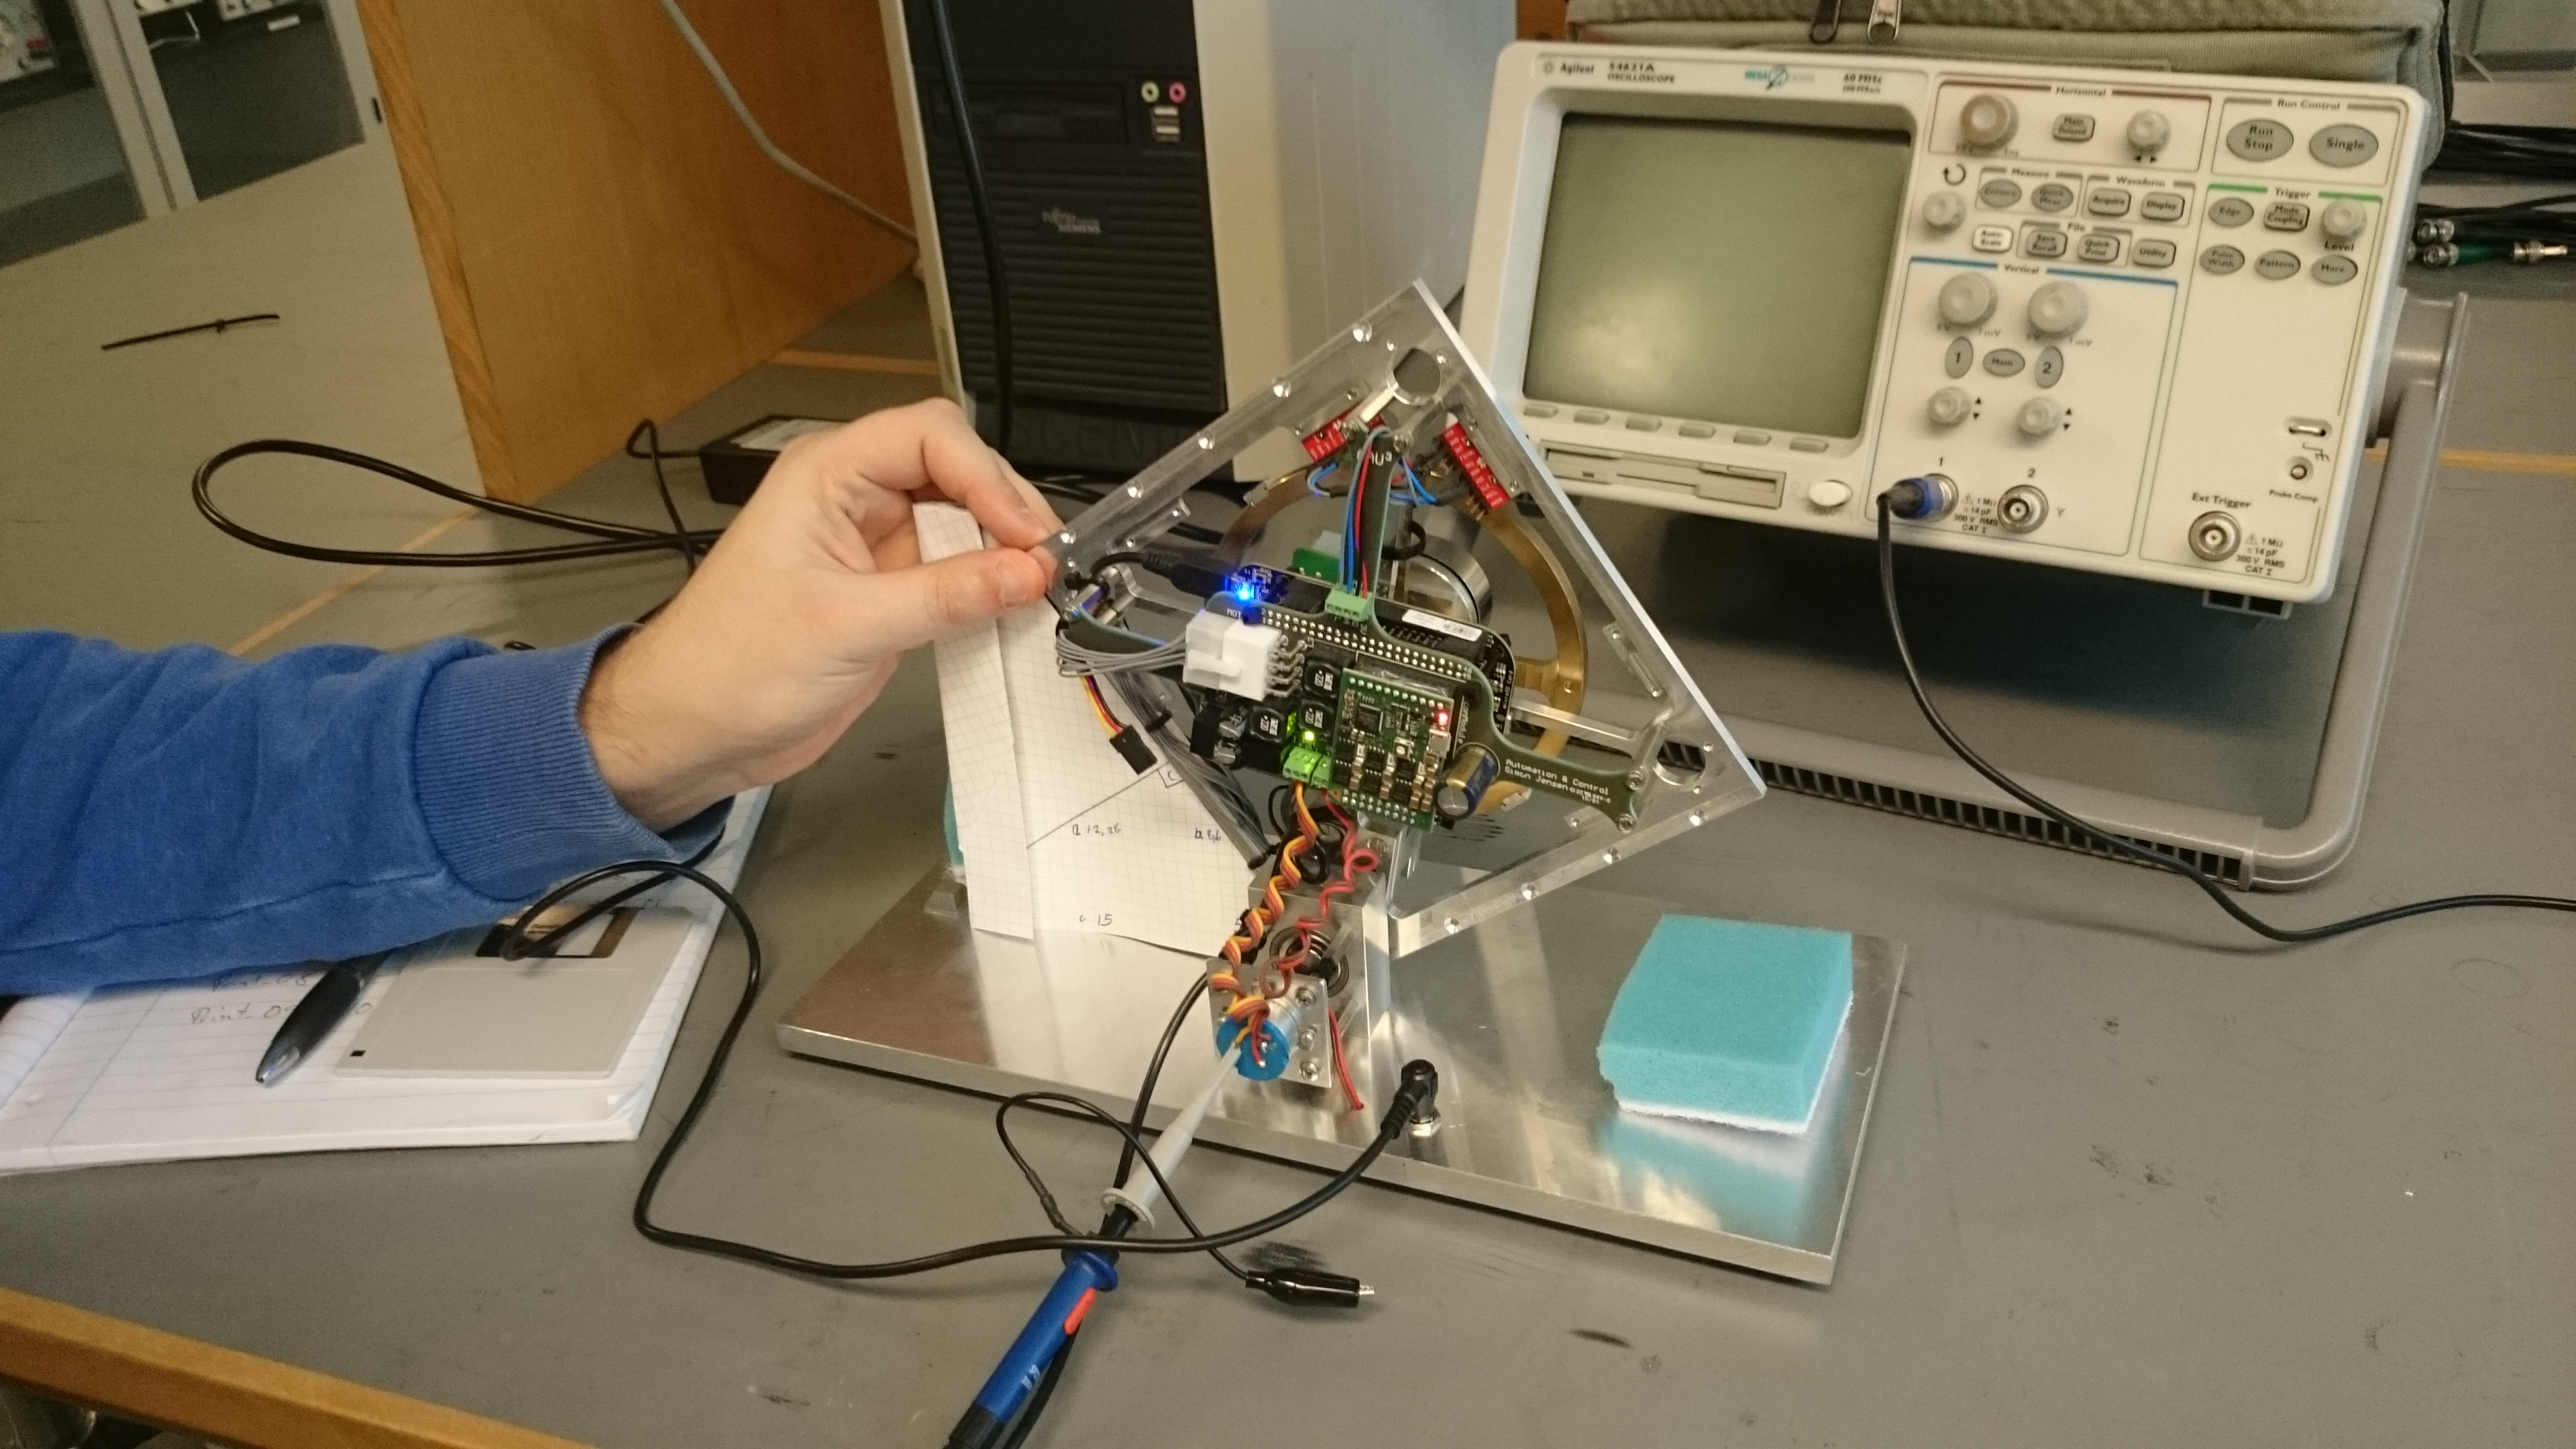
\includegraphics[scale=0.08]{figures/stepResponseSetup}
	\caption{Picture of the setup for the step-response test}
	\label{stepResponseTestPicture} 
\end{figure}              

\subsubsection{List of Equipment}
\begin{table}[H]
	\begin{tabular}{|l|l|p{4cm}|}
		\hline%------------------------------------------------------------------------------------
		\textbf{Instrument}                        &  \textbf{AAU-no.}  &  \textbf{Type}       \\
		\hline%------------------------------------------------------------------------------------
		Oscilloscope                              &  61604             &  Agilent 54621A		  \\
		\hline%------------------------------------------------------------------------------------
		Dedicated Power Supply of Cubli \small{(24 V - 3 A)} &               &  XP Power, AEB70US24 \\
		\hline%------------------------------------------------------------------------------------
		Probe 1:1                &  TBD            &          TBD\fxnote{find the probe used}    \\
		\hline%------------------------------------------------------------------------------------
		Sponge               &              &              \\
		\hline%------------------------------------------------------------------------------------
	\end{tabular}
\end{table}
>>>>>>> b5c3798a86deb9e8a1f72534e3bf37d900175072

\subsubsection{Procedure}
\begin{enumerate}
	%\item Turn on the power supply
	\item Keep the Cubli near the starting position (\si{0^\circ} or \si{10^\circ})
	\item Let the Cubli fall over
	\item Use the oscilloscope to measure the voltage changes in the potentiometer and save them
	\item Take the measurements and plot them in Matlab
	%\item Plot the result of the simulations in the same figure and compare them

\end{enumerate}

%\subsubsection{Results}
%\begin{figure}[H] 
%	\centering 
%	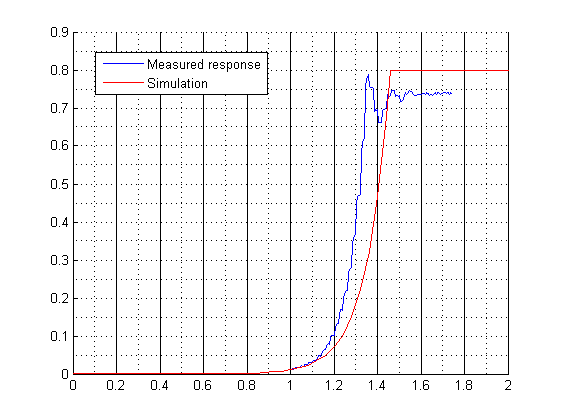
\includegraphics[scale=0.9]{figures/comparisonRealModel}
%	\caption{Comparison between the real behavior and the simulation of the linearized model}
%	\label{rawDataFallResponse}
%\end{figure} 

\begin{minipage}{\linewidth}
	\begin{minipage}{0.45\linewidth}
		\begin{figure}[H]
			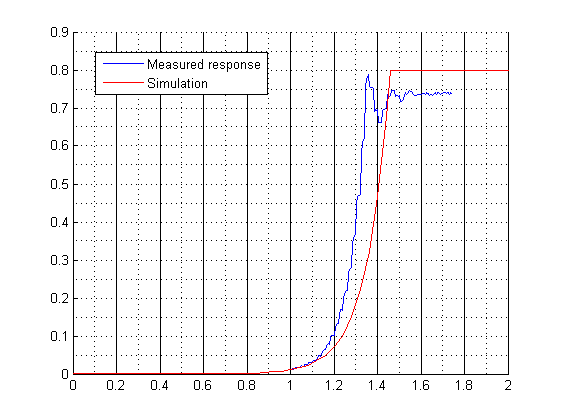
\includegraphics[scale=.53]{figures/comparisonRealModel}
			\centering
			\vspace{-.4cm}
			\captionsetup{justification=centering}
			\captionof{figure}{FIGURE 1 description}
			\label{HbridgeClokwise4Q}
		\end{figure}\vspace{-5mm}
	\end{minipage}
	\hspace{0.03\linewidth}
	\begin{minipage}{0.45\linewidth}
		\begin{figure}[H]
			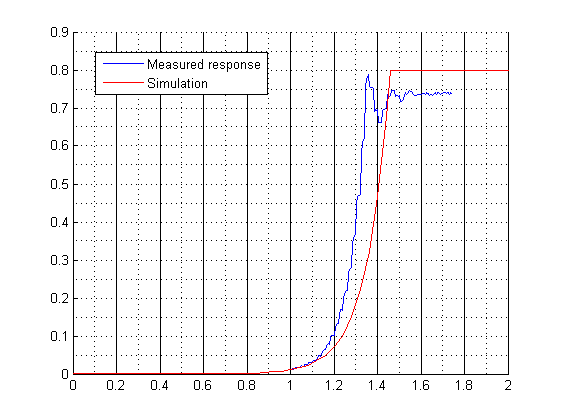
\includegraphics[scale=.53]{figures/comparisonRealModel}
			\centering
			\vspace{-.4cm}
			\captionsetup{justification=centering}
			\captionof{figure}{figure 2 description}
			\label{HbridgeCounterClokwise4Q}
		\end{figure}\vspace{-5mm}
	\end{minipage}
\end{minipage} \fxnote{Look at the layout of picture of data placement}

The data is available as a .csv file on the CD\fxnote{Make sure this is put into the CD folder for copying}

%The result of the experiment (\figref{comparisonRealModel}) shows that the response of the real system has several differences with the one from the simulation.
%
%The fist one is the presence of oscillations in the real response curve. This behavior is due to a small bounce that the frame does when it reaches the base.
%
%Another one is the final position of the frame, but it is due to the existence of a piece of foam at this position in the real case (to avoid the Cubli to hit the base).
%
%The other main difference is the shape of the curve, since the simulation is slower than the real case.

\subsubsection{Note}
Because of the sponge used as a cushion, to dampen the impact of the Cubli, there can be observed some bouncing in the data when the frame reaches the outer position.

\subsubsection{Conclusions}

